%-*- coding: utf-8 -*-

\documentclass{ICPCnotebook}
%\usepackage[UTF8]{ctex}

\title{\vspace{-4ex}\Large{ICPC Notebook}}
\author{Tifa, tan60}
\date{\today}
\bibliographystyle{plain}

\begin{document}
    \maketitle

    \pagestyle{plain}

	\pagenumbering{roman}
	\setcounter{page}{1}

    \paragraph{项目地址} \url{https://github.com/Tiphereth-A/CP-lib}

    本书代码默认数组下标从 \(0\) 开始 (\([0, n)\)), 故需注意题目下标是从 \(0\) 开始 (\([0, n)\)) 还是从 \(1\) 开始 (\([1, n]\))

    \paragraph{缺省源}

    \inputminted{cpp}{src/src/main.cpp}

    \paragraph{试机代码}

    \inputminted{cpp}{src/src/test.cpp}

    \paragraph{赛时 Clang-Format 配置}
    
    \inputminted{yaml}{src/src/.clang-format}

    \newpage
    \begin{multicols}{2}
        \tableofcontents
    \end{multicols}

    \newpage
	\pagestyle{fancy}
	\pagenumbering{arabic}
	\setcounter{page}{1}

    \input{_gen/contents_notebook.tex}
    \input{_gen/contents_cheatsheet.tex}

    \section{Theoretical Computer Science Cheat Sheet}
    \label{sec:theoretical-computer-science-cheat-sheet}

    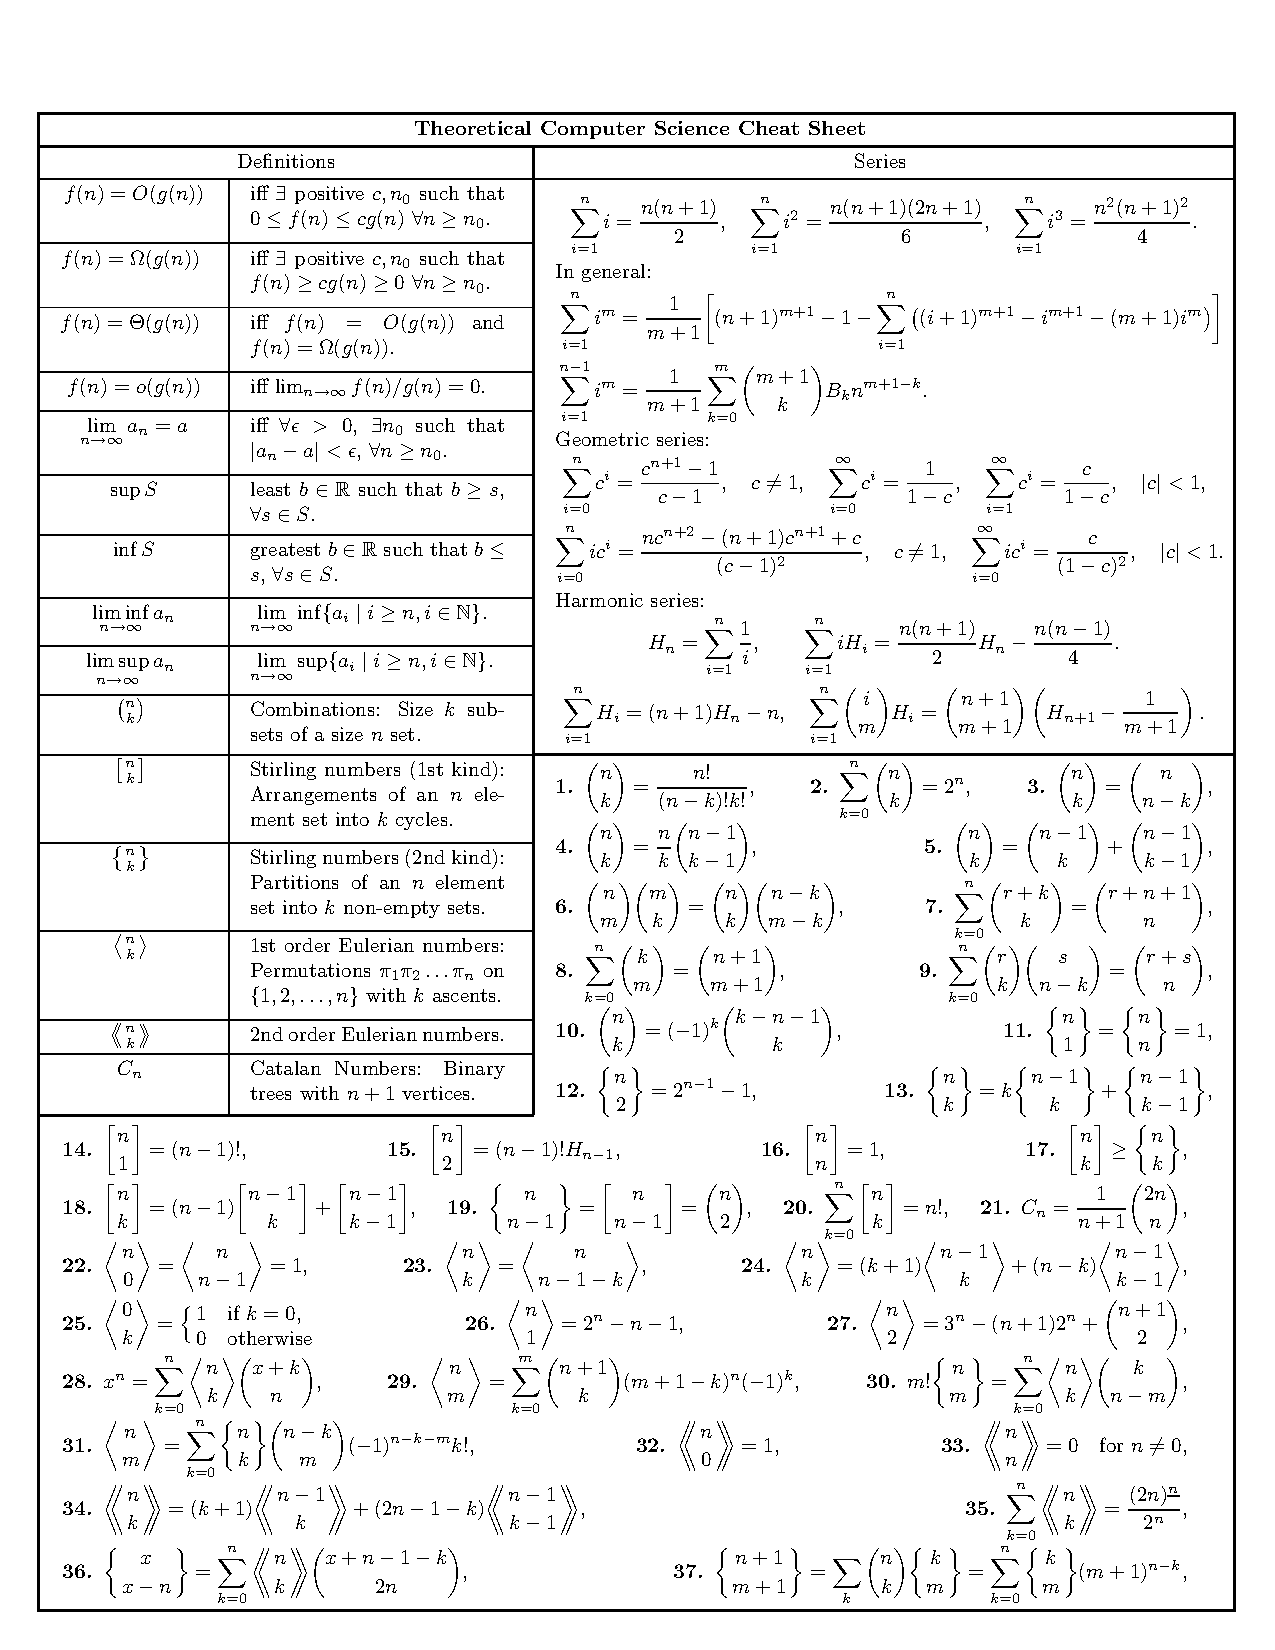
\includepdf[pages=-,pagecommand={}]{src/src/cheat.pdf}
    \bibliography{notebook}
\end{document}
